% This code uses the tikz package
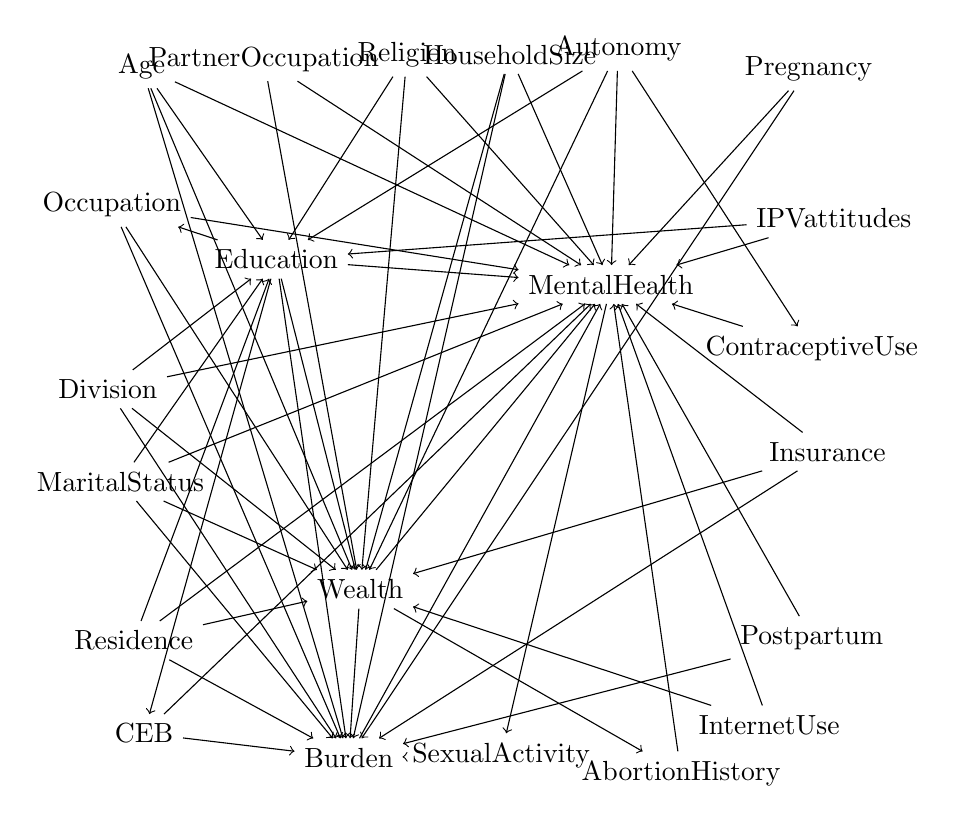
\begin{tikzpicture}
\node (v0) at (-0.915,-2.09) {Wealth};
\node (v1) at (-1.06,-4.23) {Burden};
\node (v2) at (2.27,1.78) {MentalHealth};
\node (v3) at (-1.98,2.10) {Education};
\node (v4) at (-4.07,2.79) {Occupation};
\node (v5) at (-2.14,4.64) {PartnerOccupation};
\node (v6) at (-3.69,4.55) {Age};
\node (v7) at (-3.96,-0.724) {MaritalStatus};
\node (v8) at (-4.12,0.451) {Division};
\node (v9) at (-3.79,-2.74) {Residence};
\node (v10) at (-0.320,4.70) {Religion};
\node (v11) at (-3.66,-3.92) {CEB};
\node (v12) at (0.983,4.70) {HouseholdSize};
\node (v13) at (2.36,4.77) {Autonomy};
\node (v14) at (5.10,2.62) {IPVattitudes};
\node (v15) at (5.02,-0.343) {Insurance};
\node (v16) at (4.28,-3.81) {InternetUse};
\node (v17) at (4.78,4.52) {Pregnancy};
\node (v18) at (4.82,-2.71) {Postpartum};
\node (v19) at (0.875,-4.20) {SexualActivity};
\node (v20) at (4.82,0.969) {ContraceptiveUse};
\node (v21) at (3.16,-4.43) {AbortionHistory};
\draw [->] (v6) edge (v3);
\draw [->] (v6) edge (v0);
\draw [->] (v6) edge (v1);
\draw [->] (v6) edge (v2);
\draw [->] (v7) edge (v3);
\draw [->] (v7) edge (v0);
\draw [->] (v7) edge (v1);
\draw [->] (v7) edge (v2);
\draw [->] (v8) edge (v3);
\draw [->] (v8) edge (v0);
\draw [->] (v8) edge (v1);
\draw [->] (v8) edge (v2);
\draw [->] (v9) edge (v3);
\draw [->] (v9) edge (v0);
\draw [->] (v9) edge (v1);
\draw [->] (v9) edge (v2);
\draw [->] (v10) edge (v3);
\draw [->] (v10) edge (v0);
\draw [->] (v10) edge (v2);
\draw [->] (v12) edge (v0);
\draw [->] (v12) edge (v1);
\draw [->] (v12) edge (v2);
\draw [->] (v14) edge (v3);
\draw [->] (v14) edge (v2);
\draw [->] (v15) edge (v0);
\draw [->] (v15) edge (v1);
\draw [->] (v15) edge (v2);
\draw [->] (v16) edge (v0);
\draw [->] (v16) edge (v2);
\draw [->] (v5) edge (v0);
\draw [->] (v5) edge (v2);
\draw [->] (v13) edge (v3);
\draw [->] (v13) edge (v0);
\draw [->] (v13) edge (v2);
\draw [->] (v13) edge (v20);
\draw [->] (v3) edge (v4);
\draw [->] (v4) edge (v0);
\draw [->] (v4) edge (v1);
\draw [->] (v4) edge (v2);
\draw [->] (v3) edge (v0);
\draw [->] (v3) edge (v11);
\draw [->] (v11) edge (v1);
\draw [->] (v11) edge (v2);
\draw [->] (v3) edge (v1);
\draw [->] (v3) edge (v2);
\draw [->] (v0) edge (v1);
\draw [->] (v0) edge (v2);
\draw [->] (v1) edge (v2);
\draw [->] (v17) edge (v1);
\draw [->] (v17) edge (v2);
\draw [->] (v18) edge (v1);
\draw [->] (v18) edge (v2);
\draw [->] (v20) edge (v2);
\draw [->] (v0) edge (v21);
\draw [->] (v21) edge (v2);
\draw [->] (v1) edge (v19);
\draw [->] (v2) edge (v19);
\end{tikzpicture}